\ifnum \Version=1  
% Pulled from Test 1 202305
\question[1] Consider the autonomous differential equation $\displaystyle \frac{dy}{dt}= (y-1)(y-k^2)$.  Assume $k$ can be any real number. Draw the bifurcation diagram on the axes below. That is, plot the location of the critical points versus $k$. Please label your axes.


\ifnum \Solutions=1 {\color{DarkBlue} 
        \begin{center}
        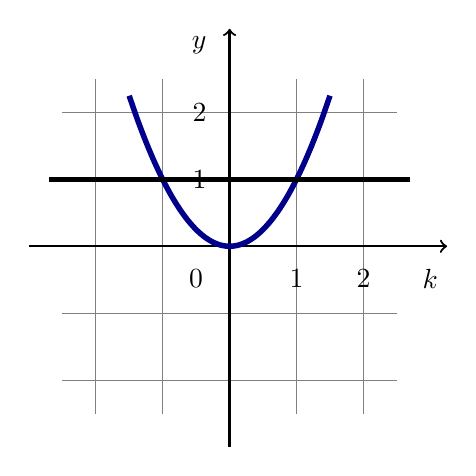
\begin{tikzpicture}[scale=0.85]
        \draw[help lines] (-2.5,-2.5) grid (2.5, 2.5);
        \draw[ thick, ->] (-3, 0) -- (3.25, 0);
        \draw[ thick, ->] (0, -3) -- (0, 3.25);
        \node[overlay, left] at (-0.2, 1) {$1$};
        \node[overlay, left] at (-0.2, 2) {$2$};
        \node[overlay, left] at (-0.2, 3) {$y$};
        \node[overlay, below] at (-0.5, -0.2) {$0$};
        \node[overlay, below] at (1, -0.2) {$1$};
        \node[overlay, below] at (2, -0.2) {$2$};
        \node[overlay, below] at (3, -0.2) {$k$};
        \draw[DarkBlue, line width = 0.70mm]   plot[smooth,domain=-1.5:1.5] (\x, {\x*\x});        
        \draw[ line width = 0.70mm, -] (-2.7, 1) -- (2.7, 1);
        
        \end{tikzpicture}
        \end{center}
} 
\else 
        \begin{center}
        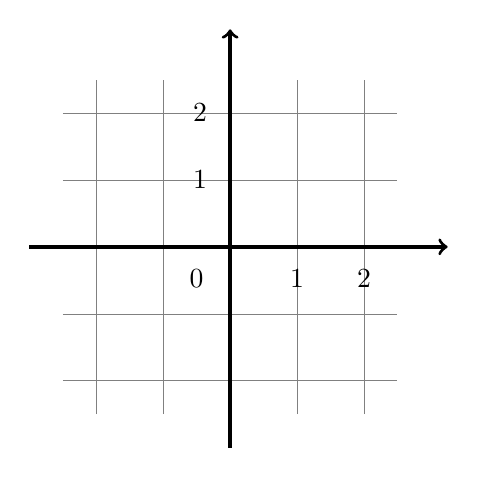
\begin{tikzpicture}[scale=0.85]
        \draw[help lines] (-2.5,-2.5) grid (2.5, 2.5);
        \draw[very thick, ->] (-3, 0) -- (3.25, 0);
        \draw[very thick, ->] (0, -3) -- (0, 3.25);
        \node[overlay, left] at (-0.2, 1) {$1$};
        \node[overlay, left] at (-0.2, 2) {$2$};
        \node[overlay, below] at (-0.5, -0.2) {$0$};
        \node[overlay, below] at (1, -0.2) {$1$};
        \node[overlay, below] at (2, -0.2) {$2$};
        \end{tikzpicture}
        \end{center}
\fi        
\fi


\ifnum \Version=2
    \question[2] You do not need to show your work for this question. Consider the differential equation 
    \begin{align*}
        2y'' - 4ty' + 3y = 9
    \end{align*}
    The DE can be expressed in the form $\vec x\, ' = A\vec x + \vec g$, where 
    \begin{align*}
     A = \left( \hbox to 2cm{\vbox to 0.85cm{}} \right), \quad \vec g = \left( \hbox to 1.2cm{\vbox to 0.85cm{}} \right)
    \end{align*}
    Fill in the missing entries in the above to define $A$ and $\vec g$. 
    \ifnum \Solutions=1 {\color{DarkBlue} \\[12pt] 
    Solve for $y''$ to obtain
    $$y'' = 2ty'-\frac32y+\frac92$$
    Then set $x_1 = y$, and $x_2 = y'$, so
    $$A = \begin{pmatrix} 0&1\\-3/2&2t\end{pmatrix}, \quad g = \begin{pmatrix} 0\\9/2\end{pmatrix}$$
    } 
    \else 
    \fi    
\fi



\ifnum \Version=3
    \question[2] You do not need to show your work for this question. Consider the differential equation 
    \begin{align*}
        2y'' - 7y' + 8ty = 4\cos(t)
    \end{align*}
    The DE can be expressed in the form $\vec x\, ' = A\vec x + \vec g$, where 
    \begin{align*}
     A = \left( \hbox to 2cm{\vbox to 0.85cm{}} \right), \quad \vec g = \left( \hbox to 1.2cm{\vbox to 0.85cm{}} \right)
    \end{align*}
    Fill in the missing entries in the above to define $A$ and $\vec g$. 
    \ifnum \Solutions=1 {\color{DarkBlue} \\[12pt] 
    $$A = \begin{pmatrix} 0&1\\-4t& 7/2\end{pmatrix}, g = \begin{pmatrix} 0\\2\cos(t)\end{pmatrix}$$
    } 
    \else 
    \fi    
\fi



\ifnum \Version=4
    \question[2] You do not need to show your work for this question. Consider the differential equation 
    \begin{align*}
        2y''' + 4y'' - 12y'  - 5y = 4\cos(t)
    \end{align*}
    The DE can be expressed in the form $\vec x\, ' = A\vec x + \vec g$, where 
    \begin{align*}
     A = \left( \hbox to 2cm{\vbox to 0.85cm{}} \right), \quad \vec g = \left( \hbox to 1.2cm{\vbox to 0.85cm{}} \right)
    \end{align*}
    Fill in the missing entries in the above to define $A$ and $\vec g$. 
    \ifnum \Solutions=1 {\color{DarkBlue} \\[12pt] 
    Solve for $y'''$ to obtain
    \begin{align}
        y''' = - 2y'' + 6y' + \frac{5}{2}y + 2\cos t
    \end{align}
    Then using
    \begin{align}
        x_1 & = y \\
        x_2 &= y' \\
        x_3 &= y''
    \end{align}
    We obtain 
    \begin{align}
        y' &= x_1 ' = x_2 \\
        y'' &= x_2' = x_3 \\
        y''' & = x_3 ' = \frac{5}{2}x_1 + 6 x_2 - 2x_3 + 2\cos t
    \end{align}
    Thus
    $$A = \begin{pmatrix} 0&1&0\\0&0&1\\\frac52& 6 & -2\end{pmatrix}, \quad \vec g = \begin{pmatrix} 0\\0\\2\cos(t)\end{pmatrix}$$
    } 
    \else 
    \fi    
\fi

\ifnum \Version>5

\question[1] Consider the autonomous differential equation $\displaystyle \frac{dy}{dt}= (y-1-k)(y-k^2)$.  Assume $k$ can be any real number. Draw the bifurcation diagram on the axes below. That is, plot the location of the critical points versus $k$. Please label your axes.


\ifnum \Solutions=1 {\color{DarkBlue} 
        \begin{center}
        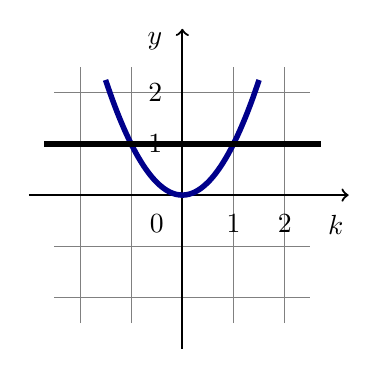
\begin{tikzpicture}[scale=0.65]
        \draw[help lines] (-2.5,-2.5) grid (2.5, 2.5);
        \draw[ thick, ->] (-3, 0) -- (3.25, 0);
        \draw[ thick, ->] (0, -3) -- (0, 3.25);
        \node[overlay, left] at (-0.2, 1) {$1$};
        \node[overlay, left] at (-0.2, 2) {$2$};
        \node[overlay, left] at (-0.2, 3) {$y$};
        \node[overlay, below] at (-0.5, -0.2) {$0$};
        \node[overlay, below] at (1, -0.2) {$1$};
        \node[overlay, below] at (2, -0.2) {$2$};
        \node[overlay, below] at (3, -0.2) {$k$};
        \draw[DarkBlue, line width = 0.70mm]   plot[smooth,domain=-1.5:1.5] (\x, {\x*\x});        
        \draw[ line width = 0.70mm, -] (-2.7, 1) -- (2.7, 1);
        
        \end{tikzpicture}
        \end{center}
} 
\else 
        \begin{center}
        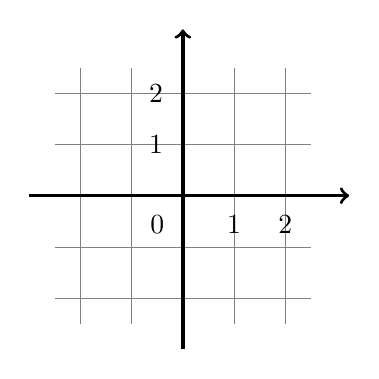
\begin{tikzpicture}[scale=0.65]
        \draw[help lines] (-2.5,-2.5) grid (2.5, 2.5);
        \draw[very thick, ->] (-3, 0) -- (3.25, 0);
        \draw[very thick, ->] (0, -3) -- (0, 3.25);
        \node[overlay, left] at (-0.2, 1) {$1$};
        \node[overlay, left] at (-0.2, 2) {$2$};
        \node[overlay, below] at (-0.5, -0.2) {$0$};
        \node[overlay, below] at (1, -0.2) {$1$};
        \node[overlay, below] at (2, -0.2) {$2$};
        \end{tikzpicture}
        \end{center}
\fi        
\fi